% Lecture Template for ME3050-001-002-Tristan Hill - Spring 2020 - Summer
% Dynamics Modeling and Controls
% Higher Order Systems - Modeul 13 - Topic 3

% I am finally converting my stuff to BEAMER

% Document settings

%\documentclass{beamer}                  % for presentation ?
\documentclass[handout]{beamer}  % for handout ?
\usepackage{beamerthemesplit}
\usepackage{amsmath}
\usepackage{listings}
\usepackage{multicol}
\usepackage{framed}
\usepackage{amsmath, nccmath}
\usepackage{geometry}
\usepackage{bm}


\beamertemplateballitem

\definecolor{TTUpurple}{rgb}{0.3098, 0.1607, 0.5176} % TTU Purple (primary)
\definecolor{TTUgold}{rgb}{1.0000, 0.8666, 0.0000} % TTU Gold (primary)

\setbeamercolor{palette primary}{bg=TTUpurple,fg=TTUgold}
\setbeamercolor{palette secondary}{bg=black,fg=TTUgold}
\setbeamercolor{palette tertiary}{bg=black,fg=TTUpurple}
\setbeamercolor{palette quaternary}{bg=TTUgold,fg=black}
\setbeamercolor{structure}{fg=TTUpurple} % itemize, enumerate, etc
\setbeamercolor{section in toc}{fg=TTUpurple} % TOC sections

% custom colors
\definecolor{TTUpurple}{rgb}{0.3098, 0.1607, 0.5176} % TTU Purple (primary)
\definecolor{TTUgold}{rgb}{1.0000, 0.8666, 0.0000} % TTU Gold (primary) 
\definecolor{mygray}{rgb}{.6, .6, .6}
\definecolor{mypurple}{rgb}{0.6,0.1961,0.8}
\definecolor{mybrown}{rgb}{0.5451,0.2706,0.0745}
\definecolor{mygreen}{rgb}{0, .39, 0}
\definecolor{mypink}{rgb}{0.9960, 0, 0.9960}

% color commands
\newcommand{\R}{\color{red}}
\newcommand{\B}{\color{blue}}
\newcommand{\BR}{\color{mybrown}}
\newcommand{\K}{\color{black}}
\newcommand{\G}{\color{mygreen}}
\newcommand{\PR}{\color{mypurple}}
\newcommand{\PN}{\color{mypink}}
\newcommand{\OR}{\color{TTU}}
\newcommand{\GD}{\color{TTUgold}}


\newcommand{\Lagr}{\mathcal{L}} % lagrangian

\newcommand{\hspcu}{\underline{\hspace{20mm}}} % large horizontal space w underline
\newcommand{\vspccc}{\vspace{6mm}\\} % large vertical space
\newcommand{\vspcc}{\vspace{4mm}\\}   % medium vertical space
\newcommand{\vspc}{\vspace{2mm}\\}     % small vertical space

\newcommand{\hspcccc}{\hspace{10mm}} % large horizontal space
\newcommand{\hspccc}{\hspace{6mm}} % large horizontal space
\newcommand{\hspcc}{\hspace{4mm}}   % medium horizontal space
\newcommand{\hspc}{\hspace{2mm}}     % small horizontal space

\newsavebox{\mybox} % custom box

\newcommand{\MNUM}{13\hspace{2mm}} % Module number
\newcommand{\TNUM}{3\hspace{2mm}} % Topic number 
\newcommand{\moduletitle}{Higher Order Systems} % Titles and Stuff
\newcommand{\topictitle}{2DOF State Space} 

\newcommand{\sectiontitleI}{Equation Decomposition} % More Titles and Stuff
\newcommand{\sectiontitleII}{State Space Equation}
\newcommand{\sectiontitleIII}{Output Equation}
\newcommand{\sectiontitleIV}{---}

\author{ME3050 - Dynamics Modeling and Controls}
\title{Module \MNUM - \moduletitle}
\date{Mechanical Engineering\vspc Tennessee Technological University}

\begin{document}

\lstset{language=MATLAB,basicstyle=\ttfamily\small,showstringspaces=false}

\frame{\titlepage \center\begin{framed}\Large \textbf{Topic \TNUM - \topictitle}\end{framed} \vspace{5mm}}

% Section 0 - Outline
\frame{
	
	\large \textbf{Topic \TNUM - \topictitle} \vspace{3mm}\\
	
	\begin{itemize}
	
		\item \sectiontitleI    \vspc % Section I
		\item \sectiontitleII 	\vspc % Section II
		\item \sectiontitleIII 	\vspc %Section III
		\item \sectiontitleIV 	\vspc %Section IV
	
	\end{itemize}

}


\section{\sectiontitleI}

\frame{ \small
  \frametitle{\sectiontitleI}

	Begin with the model and EOM we derived previously. \vspc   
	
	\begin{multicols}{2}  
  
		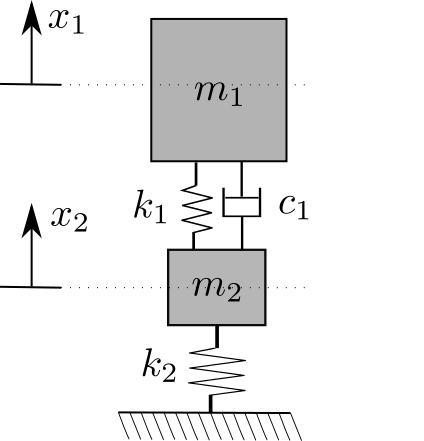
\includegraphics[scale=.4]{mass_spring_2dof.png}\\
    	\begin{fleqn}
		Equation of Motion for Mass 1: \\		
		\[ m_1\ddot{x}_1+c_1(\dot{x}_1-\dot{x}_2)+k_1(x_1-x_2)=0 \] 	
		Equation of Motion for Mass 2: \\	
		\[ m_2\ddot{x}_2+k_2x_2-c_1(\dot{x}_1-\dot{x}_2)-k_1(x_1-x_2)=0 \]\\
		\end{fleqn}
	\end{multicols}

}


\frame{  
  \frametitle{\sectiontitleI}

	Make a substitution for each dependent variable and its first derivative then re-write the system of equations as four first order differential equations. \vspccc
	let $ z_1=x_1$ and $z_2=x_2$ \vspc
	also $z_3=\dot{x}_1$ and $z_4=\dot{x}_2$ \vspccc
	You are choosing the {\it states} of your model during this process. 

}


\section{\sectiontitleII}

\frame{
  	\frametitle{\sectiontitleII}

	Write the the State Equation.
	\begin{fleqn}
	\[ \bm{ \dot{x} } = \bm{Ax} + \bm{Bu} \]
	\end{fleqn}
	
	
}


\frame{  
  \frametitle{\sectiontitleII}

}

\section{\sectiontitleIII}

\frame{
  \frametitle{\sectiontitleIII}
	Write the the Output Equation.
	\begin{fleqn}
	\[ \bm{ y } = \bm{Cx} + \bm{Du} \]
	\end{fleqn}
	

}


\frame{  
  \frametitle{\sectiontitleIII}

}

\section{\sectiontitleIV}

\frame{
  \frametitle{\sectiontitleIV}


}


\frame{  
  \frametitle{\sectiontitleIV}

}

% references is not a section for now, for looks and it would be a waste of space
\frame{

\frametitle{References}

\begin{itemize}
	\item System Dynamics, Palm III, Third Edition - Section 8.1 - Response of First Order Systems - pg. 475
\end{itemize}

}
\end{document}









